\documentclass[]{report}
\renewcommand\thesection{\arabic{section}}%for page numbering in arabics
\usepackage{graphicx,tabularx}%for figures and tables
\usepackage[utf8]{inputenc} %allows special characters such as ä, ö, ỳ
\usepackage[english]{babel}  %set the language to English
\usepackage[margin=1.5in]{geometry} %change page margins 
\usepackage{sectsty}%section headers

\setcounter{secnumdepth}{3}


\allsectionsfont{\sffamily\large}
\subsectionfont{\sffamily\normalsize}
\linespread{1.2}% line distance
\usepackage{lipsum}% http://ctan.org/pkg/lipsum
\usepackage{caption}%use for captions on tables
%use this exact command. The style and bibliographystyle has to be authoryear (Havard). The sorting is nyt: name, year, title so that the bibliography is sorted alphabetically. firstinits=true shortens the names: Albert Einstein -> A. Einstein
\usepackage[backend=biber,style=authoryear,bibstyle=authoryear,sorting=nyt,firstinits=true]{biblatex}
\setlength\parindent{0pt}%include this so that your paragraphs don't indent automatically
\addbibresource{ARDA-ML.bib} %this attaches your bib-file, your bibliography (must be in the same folder)
\usepackage[compact]{titlesec}%include title formatting package
\usepackage{graphicx}

\subsubsectionfont{\sffamily\small}
\setcounter{tocdepth}{5}
\setcounter{secnumdepth}{5}




% Title Page
\title{Exploring the Impact of Training Iterations on Object Detection Accuracy in Computer Vision}
\author{Louis Ferger Andrews and Paul Recker}
\date{December 18th 2023 \\Module: ARDA \\Venlo, Limburg, Netherlands}


\begin{document}
\maketitle

\begin{abstract}
This is the abstract.

\pagenumbering{roman}
\end{abstract}

\tableofcontents
\setcounter{page}{3}
%\listoffigures %UNCOMMENT IF YOU HAVE FIGURES
%\listoftables %UNCOMMENT IF YOU HAVE TABLES
\pagebreak
\pagenumbering{arabic}	
	


\section{Introduction}
The first chapter of the given investigation will provide the guiding research question that will be accompanied by background information based on the given topic. Expanding on this foundation, a hypothesis will be stated, that shall thereafter be tested during the conducted experiment, for the given investigation.  lalalalal

\subsection{Research Question}
How does the number of training iterations a machine learning algorithm is trained with affect the object detection accuracy of a computer vision program?

\subsection{Context and Background}
Computer vision, a rapidly growing field found in artificial intelligence, that enables computer systems to interpret visual data through the use of machine learning. It aims to replicate the human visual system, allowing it to identify objects found in images, pictures or live video feeds. The increased adoption of computer vision in various fields, such as medicine, automotive, education, security or agriculture, underlines its widespread utilization and adoption. This is primarily reasoned due to its significant impact on efficiency, effectiveness and the enhancement of various applications found in these fields. Hence its importance and impact on the future are continuously increasing. 

\subsubsection{Computer vision}
To comprehend how computer vision systems function, it is vital to comprehend the correlation they have with the human biological vision system. This is because computer vision systems follow the same principles as the human visual system. It is hypothesised by neurobiologists, that the brain aims to detect patterns it is familiar with to decode into objects. Hence the brain uses the eyes as sensors, capturing the surroundings to create a visual representation. The brain then analyses the representation for recognizable patterns, creating predictions about the objects present. The given familiar patterns are derived from previous encounters with similar objects(further explained in 1.2.2). Computer vision models aim to replicate this process, utilising the camera to create images of real-world properties. Following image processing, the data undergoes analysis to identify familiar patterns, allowing confident predictions about the objects depicted in the image, to be made \parencite{Hohman2020}.

\subsubsection{Machine learning }
Machine learning, within the field of artificial intelligence, is an approach that enables a program to utilise historical data to learn and train with, by recognising patterns in data. This allows the program to make future predictions by drawing upon the knowledge acquired during training with past historical data. Consequently, the program gains the ability to generate independent predictions without being explicitly programmed for specific predictions. This process replicates the biological approach of a child learning the names of new objects. When a child is confronted with an unfamiliar object, the child may attempt to predict what the object could be based on similarities with a known object, but won't be able to accurately identify the object. However,  if the child is given the name of the object and is exposed to multiple instances of the given object, the child will start learning and become more adept at recognizing and identifying the object when encountered again. Machine learning functions on the same basis. The more the program is trained, the more refined its predictions become, as it accumulates experiences in accurately predicting specific objects. This learning process, also referred to as machine learning training, enhances the program's ability to create accurate predictions over time. 

\subsubsection{Importance of accuracy in computer vision programs}
With the widespread integration of computer vision programs across various fields, the accuracy of the given models assumes a key significance. Tesla, an automotive market leader for self-driving cars, has widely adopted computer vision programs based on machine learning for their autonomous vehicles. It is crucial for the given programs to accurately identify objects with a high level of confidence in real-time, enabling it to create a picture of the environment it is operating in. Hence resulting in a close-to-perfect detection accuracy. The significance lies in the fact that a failure to identify an object, can result in real-world consequences such as a collision with a different object. Therefore accuracy is a pivotal aspect of computer vision programs for widespread acceptance. Furthermore recognising that a low accuracy will directly translate into high error rates in programs utilising computer vision and retrospectively resulting in potential catastrophic implications. Therefore it can be stated that the accuracy of computer vision programs based on machine learning plays a pivotal role in the practical implementation of such models in real-world applications. 


\subsection{Hypothesis}
Based on the context provided, it can be hypothesised that increasing the training iterations for the machine learning algorithm will have a direct correlation with the accuracy of the object detection model. Hence the greater the number of training iterations the program goes through, the greater the accuracy should become. This hypothesis is based on the fact that each additional iteration of training, will allow the model to converge towards a more optimised state by adjusting its parameters to minimize the differences between the training and the test data.\\


It is expected that during the initial training phases of the given experiment, specifically between 1,000 and 3,000 iterations, the model might face challenges in identifying objects in the test images accurately. In the cases where it does recognise the given objects, it is probable that it will do so with only a minimal degree of accuracy. This is thereafter expected to greatly change as the model rapidly begins to gain a basic understanding of the objects it is confronted with based on its training. Therefore it is appropriate to assume that during the stage, between  4,000 and 13,000 the greatest increase in accuracy should be displayed.  Beyond this point, it can be expected that as the model reaches a substantial accuracy of around 80\%, it can be hypothesised that the growth in accuracy will steadily decrease as the model converges towards an optimal state and the accuracy plateaus.\\


Furthermore, it can be theorised that a decrease in the model's loss should lead to an increase in accuracy, considering the inverse relationship between loss and accuracy, where a loss reduction indicates an improved performance as loss is measured by testing for accuracy.\\


In summary, a significant correlation between the accuracy and the number of training iterations for the machine learning algorithm is expected, which will gradually decrease as the model approaches its optimal state.


 
\section{Methods}
This chapter covers the methodology used to conduct the experiment which is the main focus of this paper.
It will cover the research design, the experiment setup and execution, as well as the data transformation 
and visualisation.\\

\subsection{Research Design}
The research of this paper is based on empirical and quantitative data collected from an experiment.
The experiment is made up of the following variables, the independent variable, the number of training iterations the
program is trained with, and the dependent variable, the accuracy of the model. To make sure results are accurate and consistent, 
all iterations will use the same machine learning algorithm,
the same dataset, the same evaluation data, and run on the same hardware.
The data which is being collected and analyzed is the number of iterations (categorical ordinal), the accuracy
and loss (continuous ratio), and the relation between them.\\

\begin{table}[h]
\centering
\begin{tabularx}{\textwidth}{|>{\hsize=.5\hsize}X|>{\hsize=1.5\hsize}X|}
\hline
\textbf{Type} & \textbf{Variable} \\
\hline
Independent Variable & 
\begin{tabular}{@{}l@{}}
\textbullet{} Number of Iterations  \\
\end{tabular} 
\\
\hline
Dependent Variable & 
\begin{tabular}{@{}l@{}}
\textbullet{} Accuracy of the Model\\
\end{tabular} 
\\
\hline
Controlled Variable & 
\begin{tabular}{@{}l@{}}
\textbullet{} Machine Learning Algorithm \\
\textbullet{} Dataset, Evaluation Data \\
\textbullet{} Hardware \\
\end{tabular} 
\\
\hline
\end{tabularx}
\caption{Key Variables of the Experiment}
\label{table:1}
\end{table}

\subsection{Experiment Setup and Execution}
The program "CreateML" from \cite{Apple} was used to carry out this experiment. It is a user-friendly and powerful 
tool that allows developers to create custom machine-learning models without the need for extensive expertise in the field.
CreateML simplified the process of creating and training an object detection model by providing a graphical user interface which 
just takes the input dataset and the desired parameters. The object detection model uses the YOLOv2 \parencite{Jaina} algorithm.
"You Only Look Once" (YOLO) is a state-of-the-art, real-time object detection algorithm introduced in 2015" \parencite{Keita2022}. 
The dataset used to train the object detection model is \citetitle{pascal2023} which is a collection of around 10000 images including classes
like persons, vehicles and animals. The experiment was run on a MacBook Air 2020 with an Apple M1 chip and 8GB of RAM. To ensure the 
result were unbaised the "Batch Size" was left on auto and the "Grid Size" was set to 13x13.\\

\newpage
Overall the model was trained 20.000 times and every 1000 iterations a snapshot of the model was taken and evaluated using
specific images. 
The classes and images chosen include: Boat, Dog, Person, Plant, Wheel (See Appendix~\ref{app:test-pictures}).
\begin{figure}[h]
  \centering
  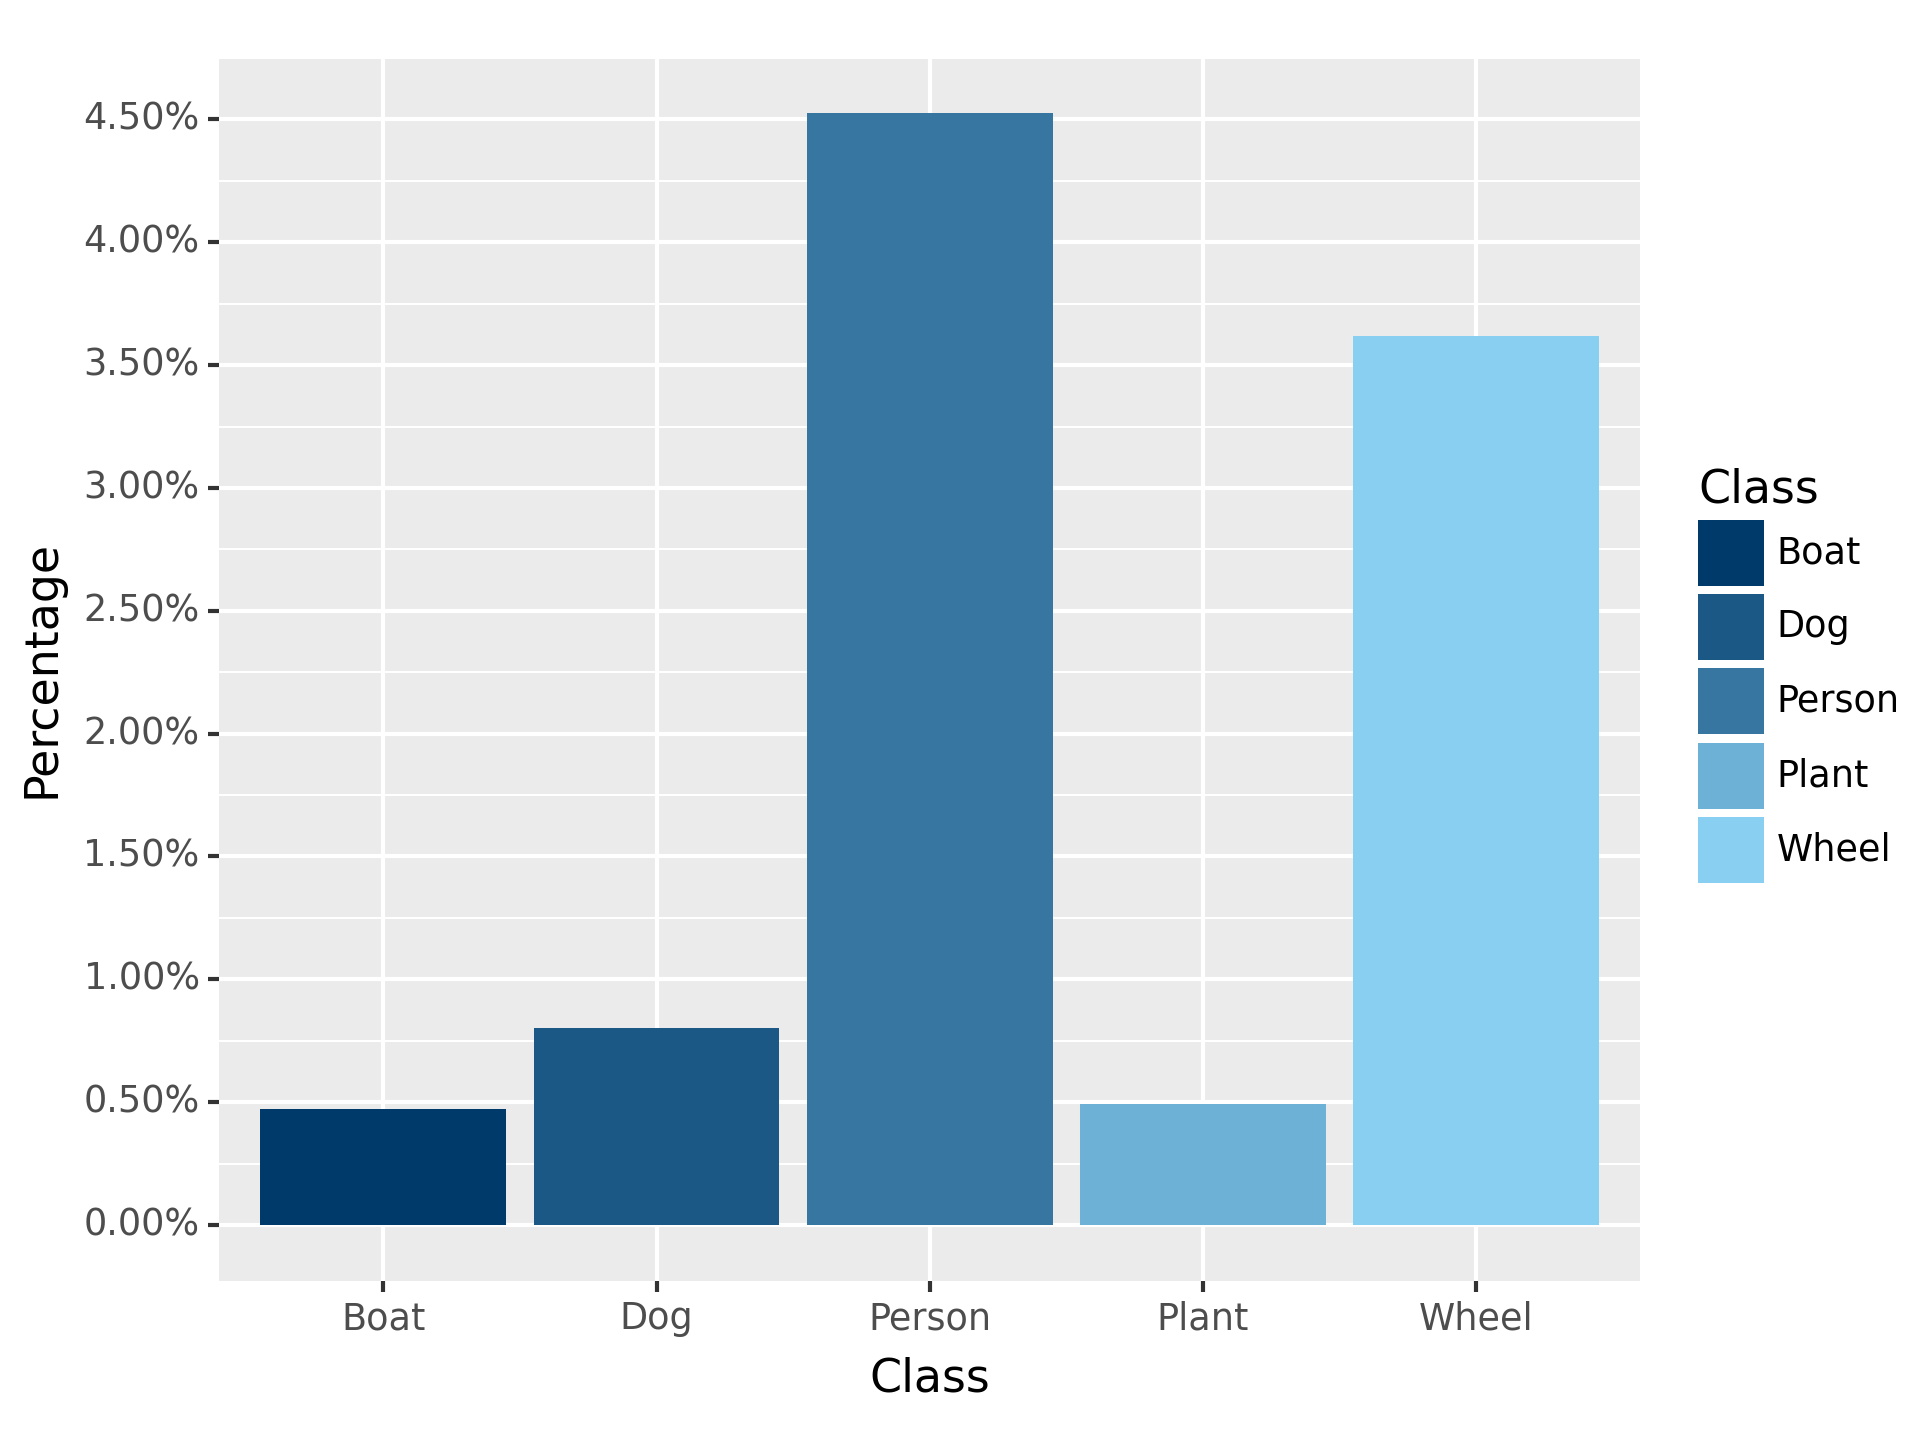
\includegraphics[width=0.70\textwidth]{../Data/distribution-classes-barchart.png}
  \caption{Class Usage in Dataset (\%)}
  \label{fig:class-usage-in-dataset}
\end{figure}
\\
Each snapshot was evaluated by using the above-mentioned images and the accuracy as well as the loss was saved in a CSV file for 
analysation.
\\
\subsection{Data Transformation and Visualisation}
Data transformation and its visualisation plays a crucial role in evaluating the hypothesis. The gathered data was exported to multiple CSV files, 
which were categorized by class and consisted of the number of iterations and the accuracy per picture. Python and Jupyter Notebooks were the
foundation for the handling of data in this project. Data manipulation was handled by Pandas and the visualisation was done using Matplotlib
and Plotnine.\\

% CLASS DISTRIBUTION
The annotations JSON file, included in the training dataset \parencite{pascal2023}, was an additional source of information. 
A custom Python script was written to transform the data into a useable format, which was required to calculate the class distribution 
and the image count per class. To illustrate which classes were evaluated and their representation in the dataset, a bar chart was created 
(See Fig.~\ref{fig:class-usage-in-dataset}). This choice was motivated by the observation that "[v]ertical bar charts are useful to compare 
different categorical [...] variables" \parencite{Statistics-Canada2021}.\\ 
\newpage

% LOSS GRAPH
The loss was graphed by using a scatter plot (See Fig.~\ref{fig:loss-vs-training-iterations})
as it visualises the relationship between two or more quantitative variables. They are especially helpful when examining whether
the values of one variable are influenced by the values of the other variable \parencite{Statistics-Canada2021b}. 
Additionally, a quadratic trend line was added to identify the trend and outliers.\\ 

% ACCURACY GRAPH
To plot the accuracy all CSV files were merged by iterating through each file, calculating the mean accuracy per iteration and appending it
to the new pandas data frame. This resulted in a data frame with the mean accuracy per iteration for each class. This data was then plotted using
a line chart (See Fig.~\ref{fig:accuracy-vs-training-iterations}). \\ 

% ACCURACY IMPROVEMENT GRAPH
To illustrate the improvement of accuracy over time, the average accuracy of all classes per iteration was calculated.
From that, the percentual increase of accuracy was calculated and then the average accuracy was plotted against the number of iterations
(See Fig.~\ref{fig:accuracy-improvement}).
A line chart was chosen for both because it is useful for illustrating trends over time \parencite{Statistics-Canada2021a}.\\

% BAR CHART FLUCTUATION WHEEL AND DOG
For further investigation into the performance of some classes, the accuracy for a specific iteration per picture was plotted 
using a line and bar chart (See Fig.~\ref{fig:14000-dog}, \ref{fig:image-1-accuracy}, \ref{fig:13000-wheel}, \ref{fig:image-3-accuracy}). 
This was done to identify outliers and to clearly display discrepancies in performance between pictures of the same class.\\

% BOX PLOT PER ITERATION
To obtain a comprehensive insight into the variation in the model's accuracies, a box plot was utilised (See. Fig~\ref{fig:Box-plot}). This visual representation illustrated the distribution of the accuracy measurements gathered during the experiment, portraying how the model evolved throughout its training process.
This graph is a good choice since its use case is illustrating the distribution of data \parencite{Tableau}.\\


\section{Results}
This chapter will focus on providing visual representations of the findings from the experiment. These findings will be described in detail to further be used to evaluate the hypothesis in the discussion section of the report. 


\subsection{Relationship between training iterations and loss}
\begin{figure}[h]
   \centering
   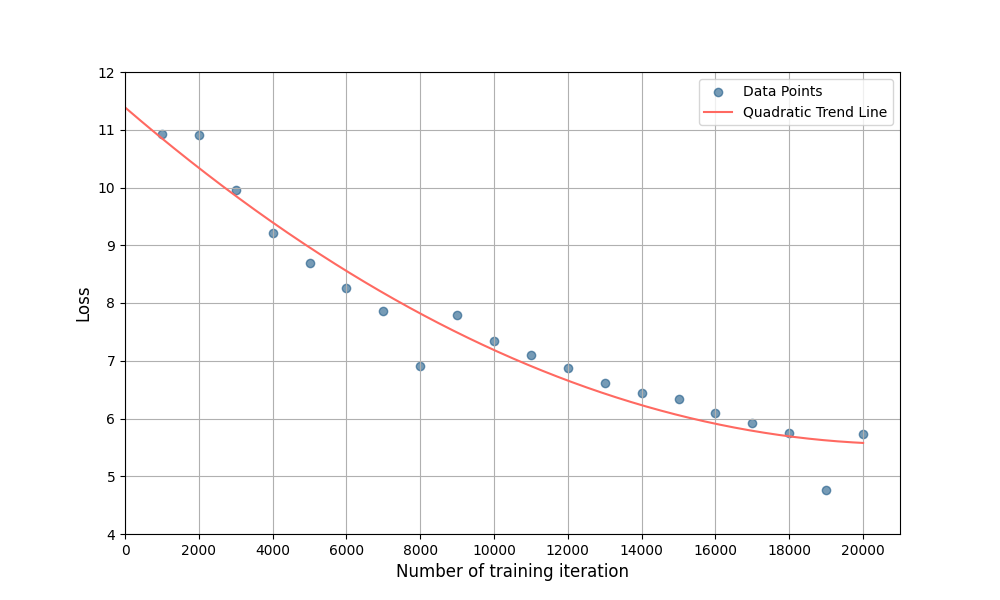
\includegraphics[width=0.9\textwidth]{../Data/loss_by_iteration_plot.png}
   \caption{Quadratic Trend Analysis of Loss Reduction Over 20,000 Training Iterations}
   \label{fig:loss-vs-training-iterations}
\end{figure}
The data illustrated in Fig.\ref{fig:loss-vs-training-iterations} displays the relationship between the the loss of the object detection model over the 20,000 training iterations of the machine learning algorithms. It can be seen that during the initial stages of the experiment, a sharp decline in the loss can be viewed. This demonstrates the initial learning phase of the program. However, with an increased number of training iterations, the rate of the loss decreasing steadily slows down as it approaches its optimal state. \\

The quadratic trendline graphed in Fig.\ref{fig:loss-vs-training-iterations}  displays the model approaching a state of convergence, as the training iteration count increases and loss decreases. Furthermore, the trendline expresses the non-linear relationship between training iterations and the loss of the model. \\
\newpage

\subsection{Relationship between training iterations and accuracy}
The accuracy per class analysis illustrates the model's learning dynamics across different classes.
Figure \ref{fig:accuracy-vs-training-iterations} displays the accuracy per class over 20,000 measured training iterations.
It can be seen that all classes, besides "Person", rapidly increase after around 2000 training iterations. After 10,000 iterations
all of these classes have an accuracy of roughly 80\%. Over the next 10,000 iterations, the accuracy then slowly approaches 95 to 100\%.
This is different for "Person", which after 1000 iterations already starts with an accuracy of about 35\% and a steep incline to 97\%
after 5500 iterations. After that it slowly approaches 100\% accuracy.
Important to note is the fluctuation of accuracy for "Dog" and "Wheel" at 13,000 and 14,000 iterations respectively.

\begin{figure}[h]
   \centering
   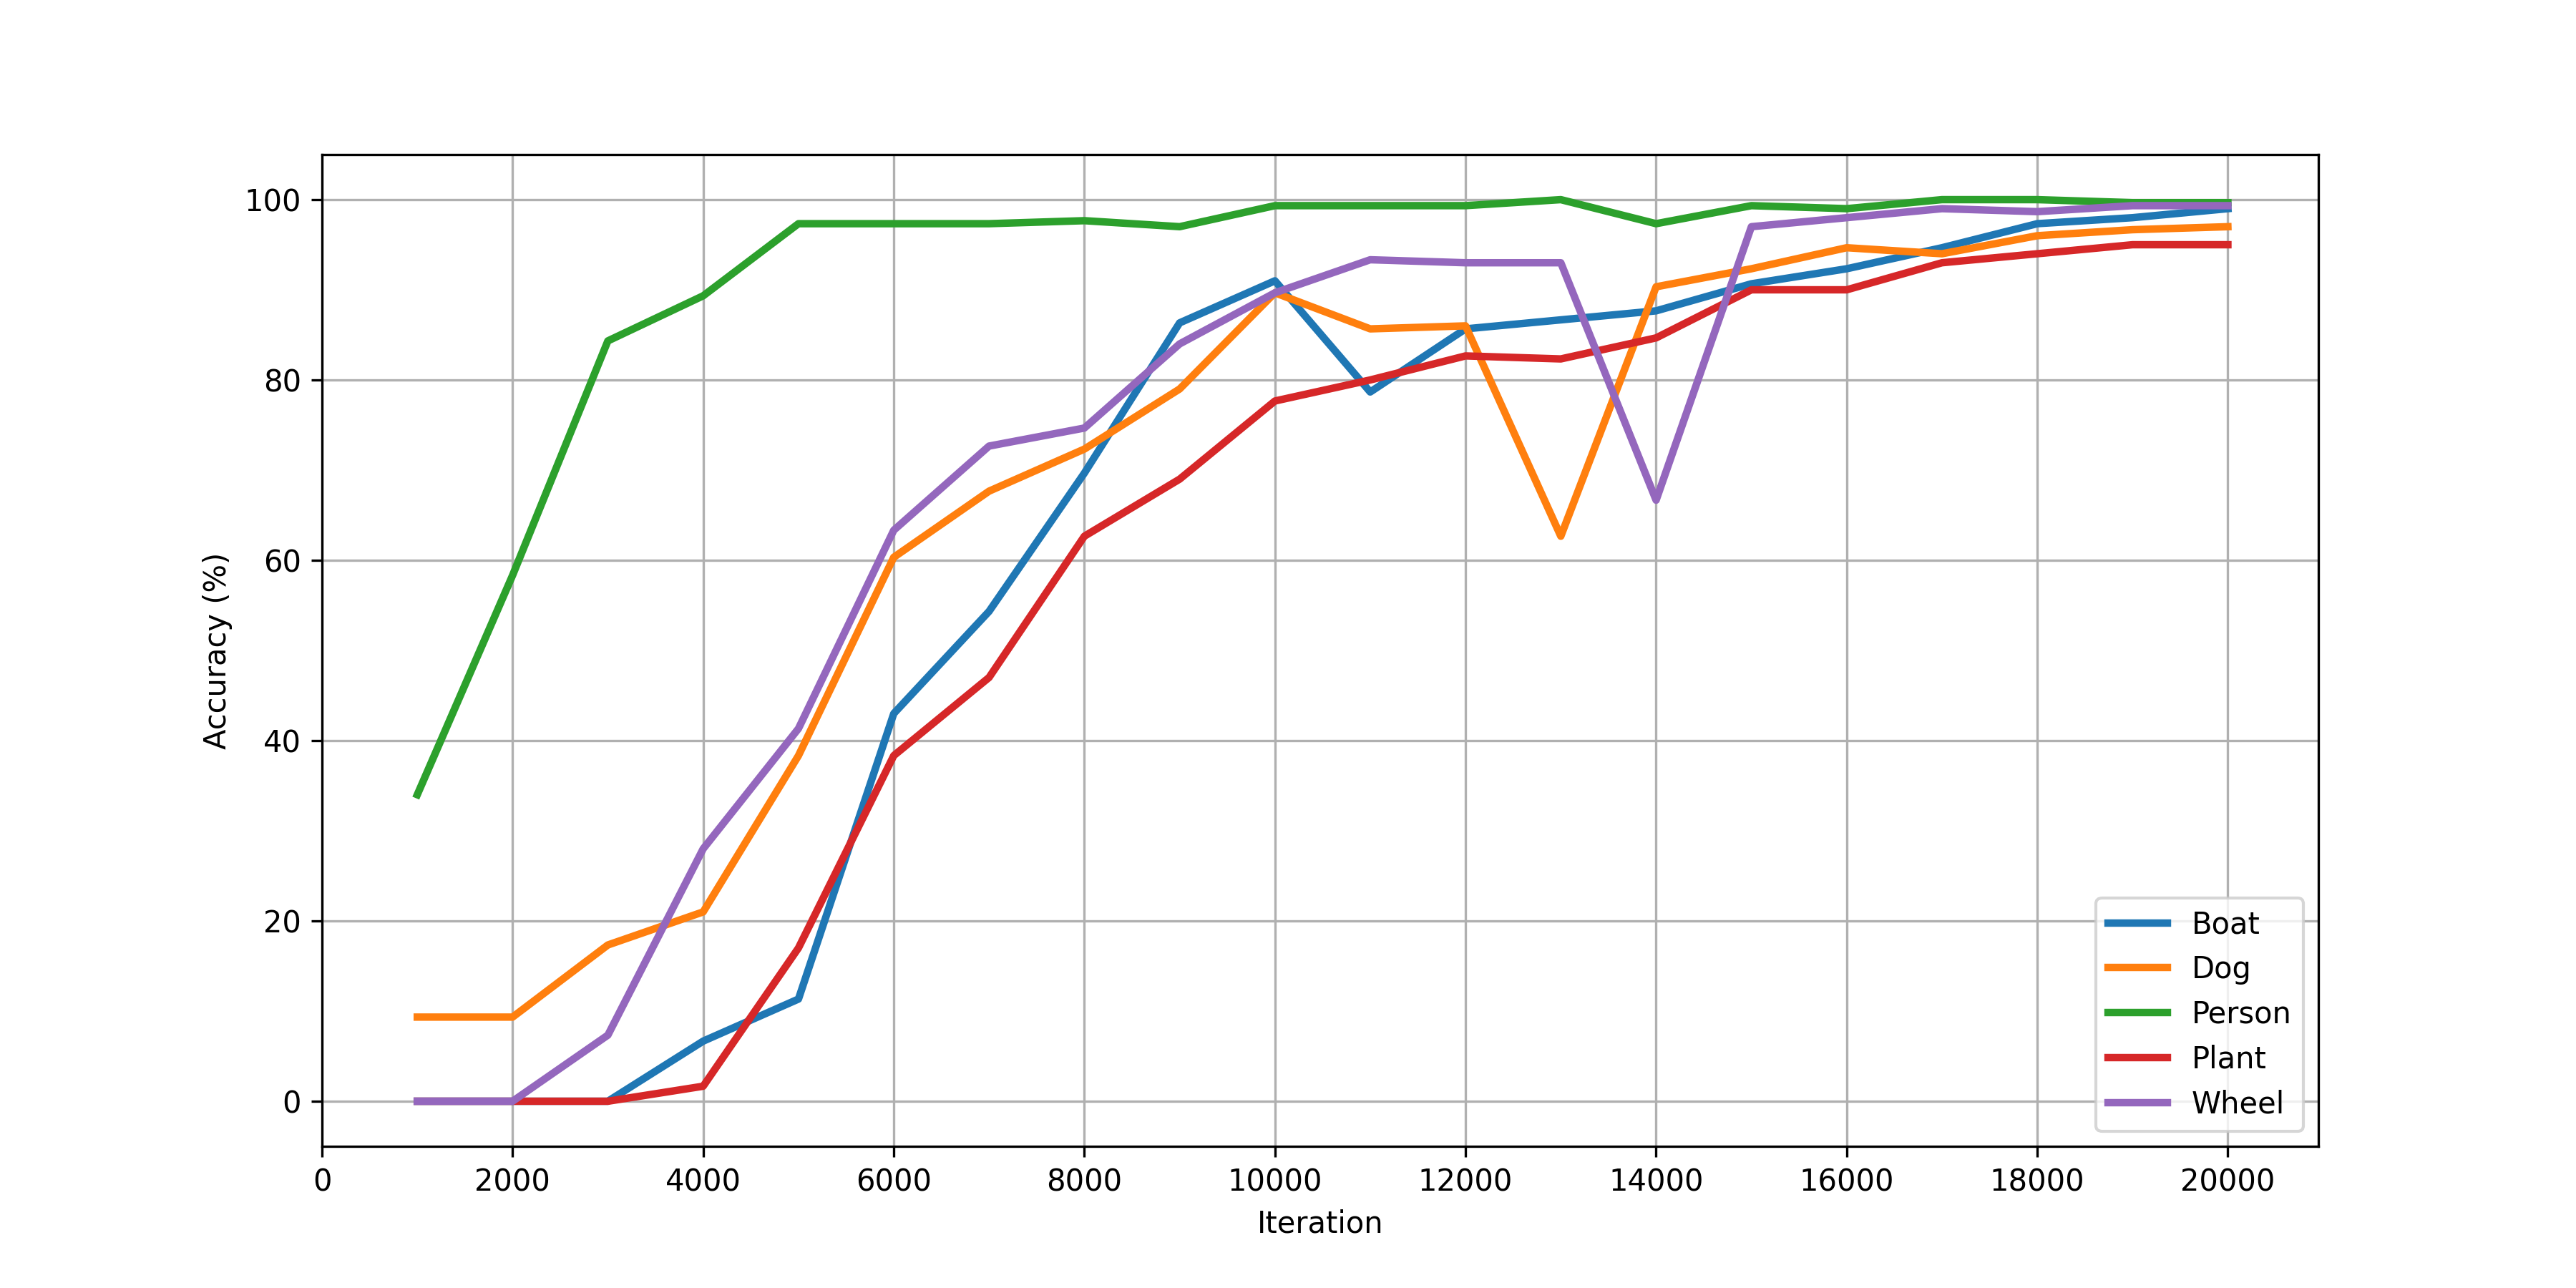
\includegraphics[width=0.9\textwidth]{../Data/accuracy-graph.png}
   \caption{Accuracy per Class over 20,000 Training Iterations}
   \label{fig:accuracy-vs-training-iterations}
\end{figure}


To assess the overall performance of the model, the average accuracy per iteration and its rate of change were calculated.
The "Average Accuracy" in Figure \ref{fig:accuracy-improvement} displays the aggregated information seen in Figure 
\ref{fig:accuracy-vs-training-iterations}. The aggregation of data attenuates the fluctuation seen for the classes "Dog" and "Wheel" 
(See Fig. \ref{fig:accuracy-vs-training-iterations}) and thus making the the upward trend between 10,000 and 20,000 iterations more visible.
\\
The model starts off with a substantial increase in accuracy, which is followed by a dip in the rate of change, as the rise in accuracy 
decelerates. A further steep incline can be detected between 4000 and 6000 iterations, which is followed by a steady increase in accuracy, as
the rate of change falls. A small dip in accuracy can be seen at iteration 11,000, after which a bigger anomaly occurs between 13,000
and 14,000 iterations. Following the dip, the model resumes its positive uptrend trend, reaching an average performance of 98\% after its final
iteration (20,000).
\newpage

\begin{figure}[h]
   \centering
   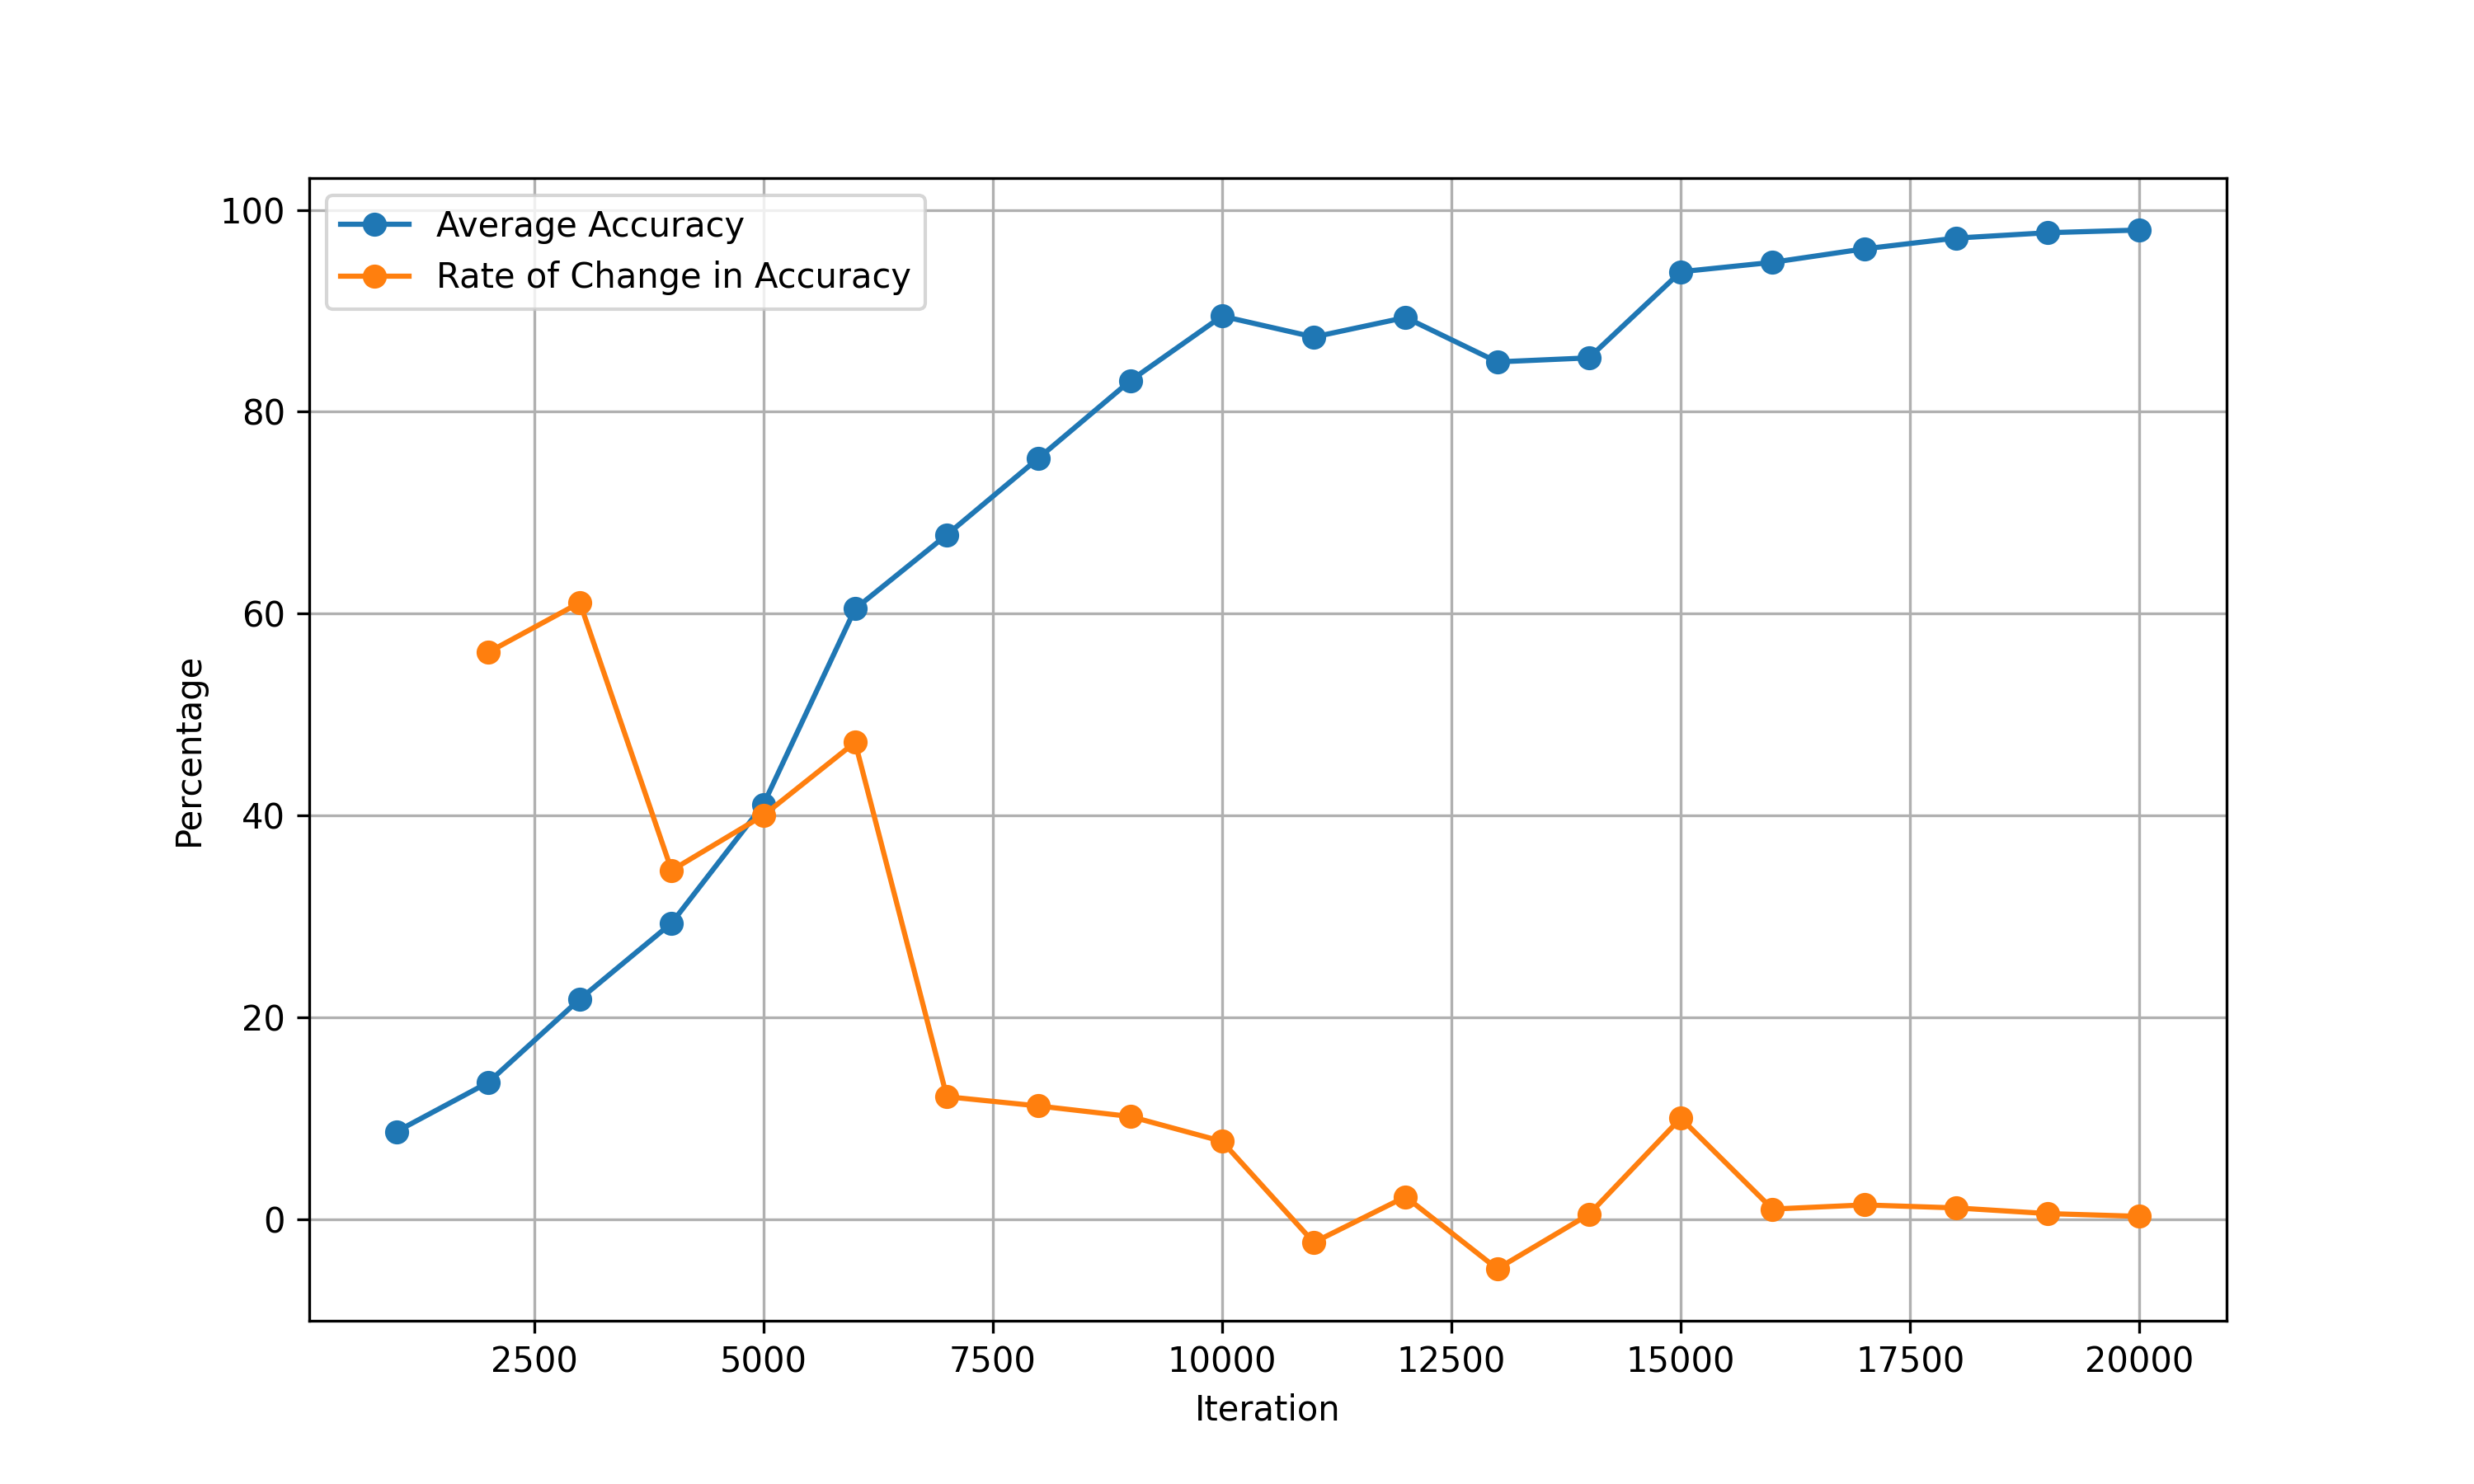
\includegraphics[width=0.9\textwidth]{../Data/accuracy-improvement-graph.png}
   \caption{Average Accuracy and its Rate of Change}
   \label{fig:accuracy-improvement}
\end{figure}

Overall, the chart depicts a generally positive trajectory for the average accuracy, with a few outliers. The "Rate of Change" emphasizes
key points in the model's learning process and makes instances in which the average accuracy experiences notable increases or decreases more
visible. The described fluctuation in accuracy needed to be further investigated, hinting at possible
challenges in the learning process of the object detection model. \\

\subsection{Analysing fluctuation in loss and accuracy}

The data reveals a notable decline in accuracy at 13,000 training iterations for the dog class and 14,000 training iterations for the wheel class, respectively. To further investigate the observed downturns in the data, analysing the average data points displaying the decline can provide a more comprehensive insight. The data points displayed in Figure (----) for each class represent the average accuracy score of three images. 
\newpage
\begin{figure}[h]
   \centering
   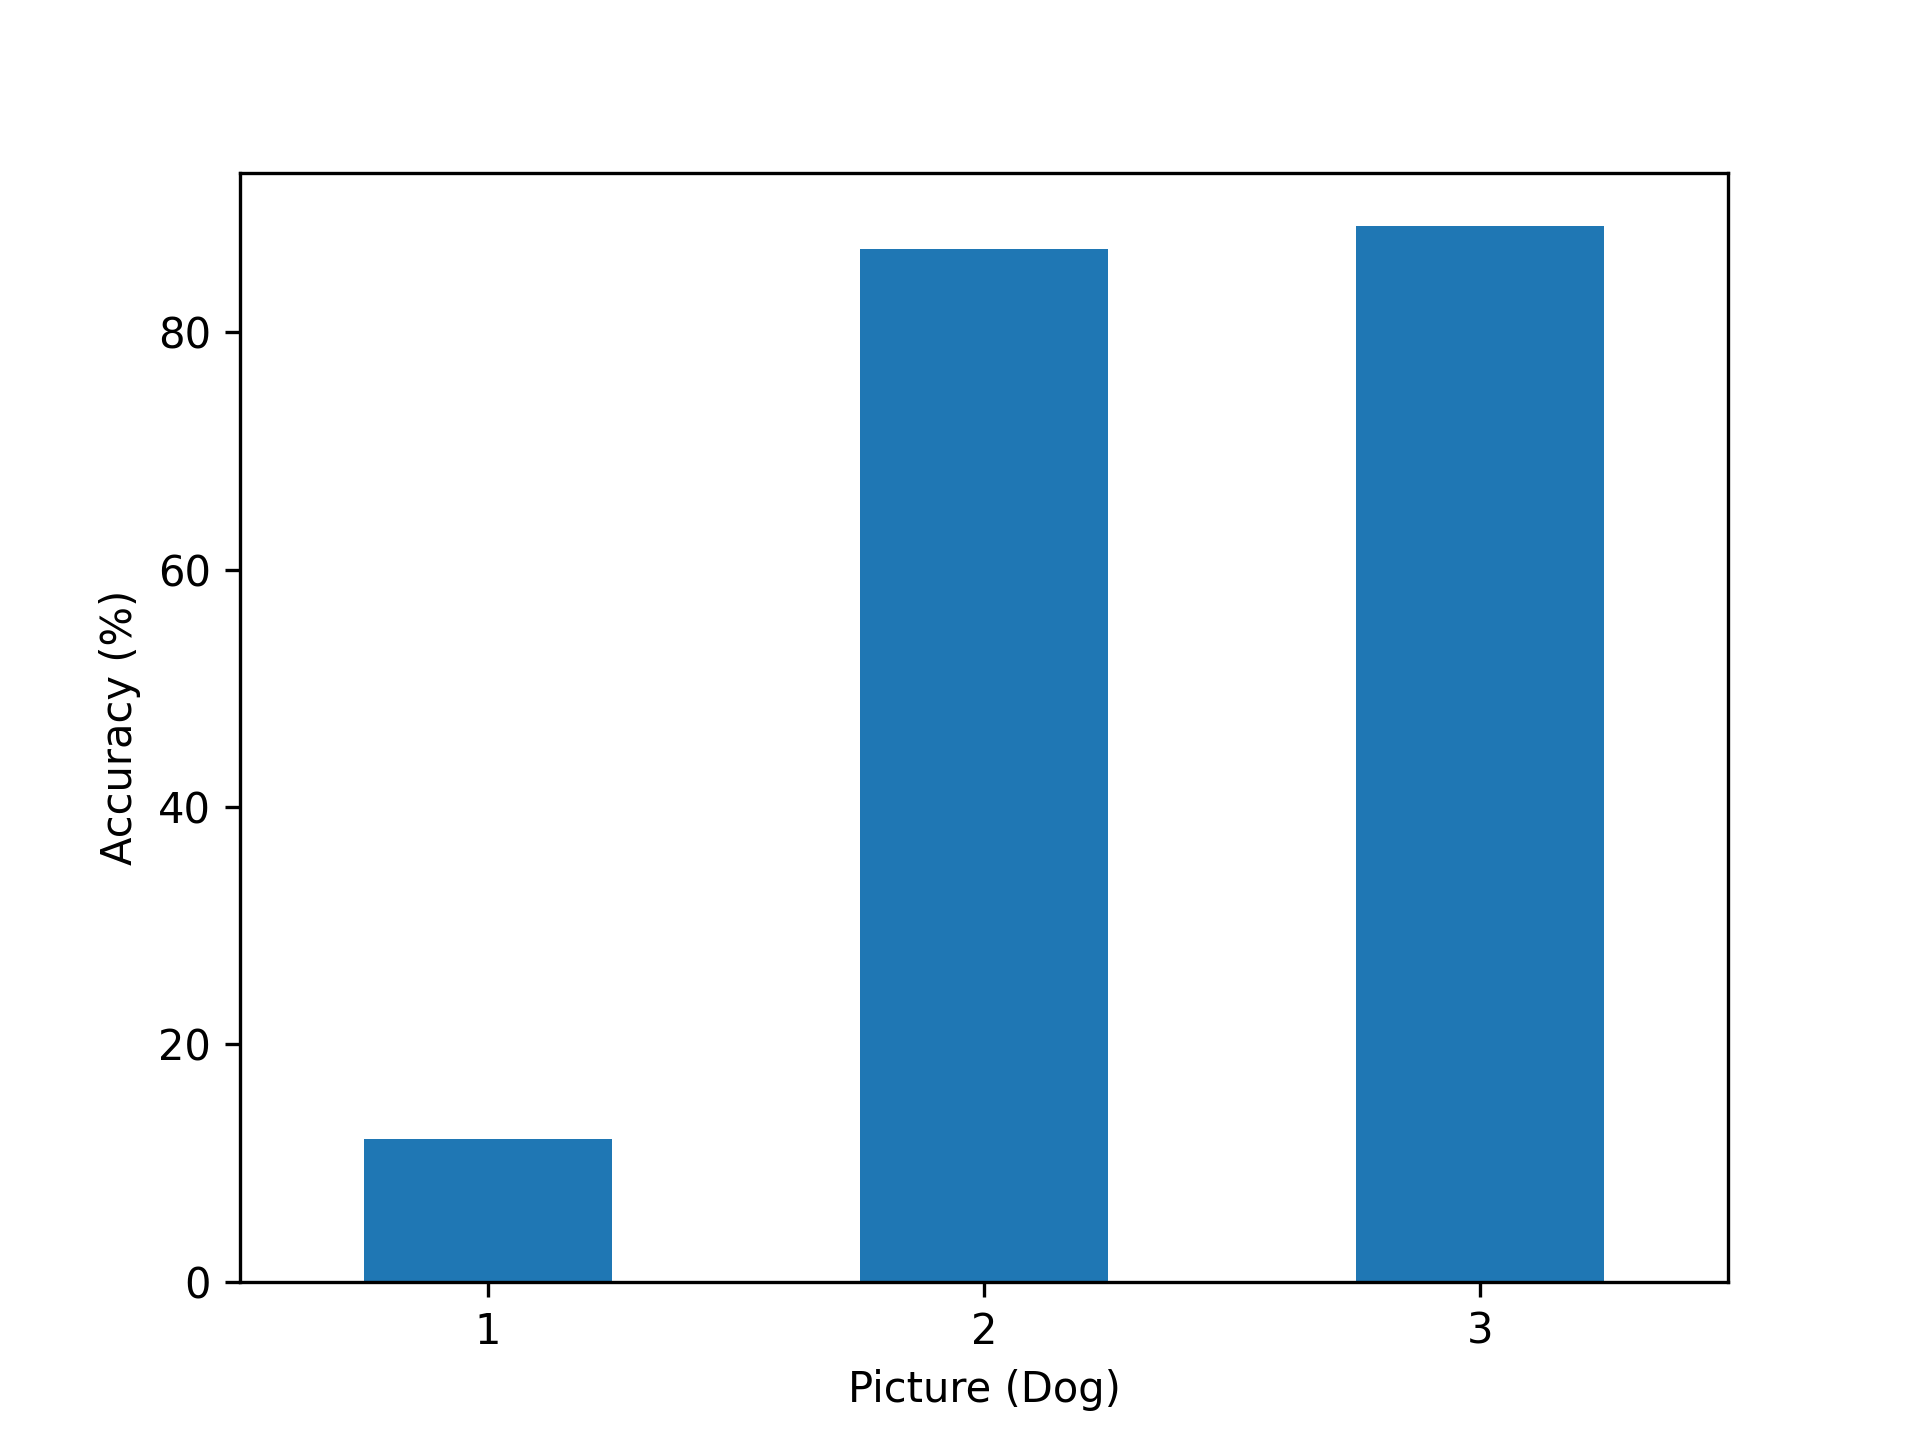
\includegraphics[width=0.5\textwidth]{../Data/dog-outliers.png}
   \caption{Accuracy Discrepancy Among Images in Dog Class at 13,000 Training Iterations}
   \label{fig:14000-dog}
\end{figure}

Figure \ref{fig:14000-dog} displays three different instances of the dog class that make up the average data point for 13,000 training iterations, at which the dip in data was observed. The graph in Figure \ref{fig:14000-dog} reveals the accuracy score obtained by each image during this iteration test. Notable both images 2 and 3 receive high accuracy scores with 87 and 89 percentage points respectively. On the other hand image 1 only has an accuracy of 12 percentage points, showing an anomaly in the data.

\begin{figure}[h]
   \centering
   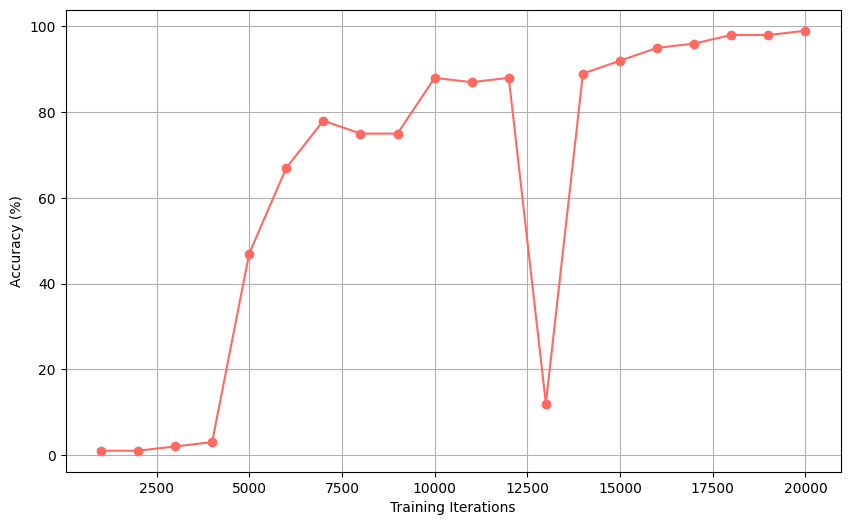
\includegraphics[width=0.5\textwidth]{../Data/dogs_image1_accuracy_vs_iteration.png}
   \caption{Dog Class Image 3 Training Iterations vs. Accuracy }
   \label{fig:image-1-accuracy}
\end{figure}

To further illustrate and investigate the dip in accuracy in the dog class, and the found anomaly in image 1,  Figure \ref{fig:image-1-accuracy} can be utilised, which displays the relationship between accuracy and training interaction for image 1. Notable in this Figure, is that the previously discovered anomaly of 12 percent at 13,000 training iterations is also clearly represented in the graph at the steep dip. This data point is a significant deviation from the otherwise existing pattern, displaying a clear divergence from the expected accuracy trajectory. Therefore it can be concluded that this data point represents an outlier in the data. Reasons for such an outlier will be evaluated in the discussion chapter. 
\newpage

\begin{figure}[h]
   \centering
   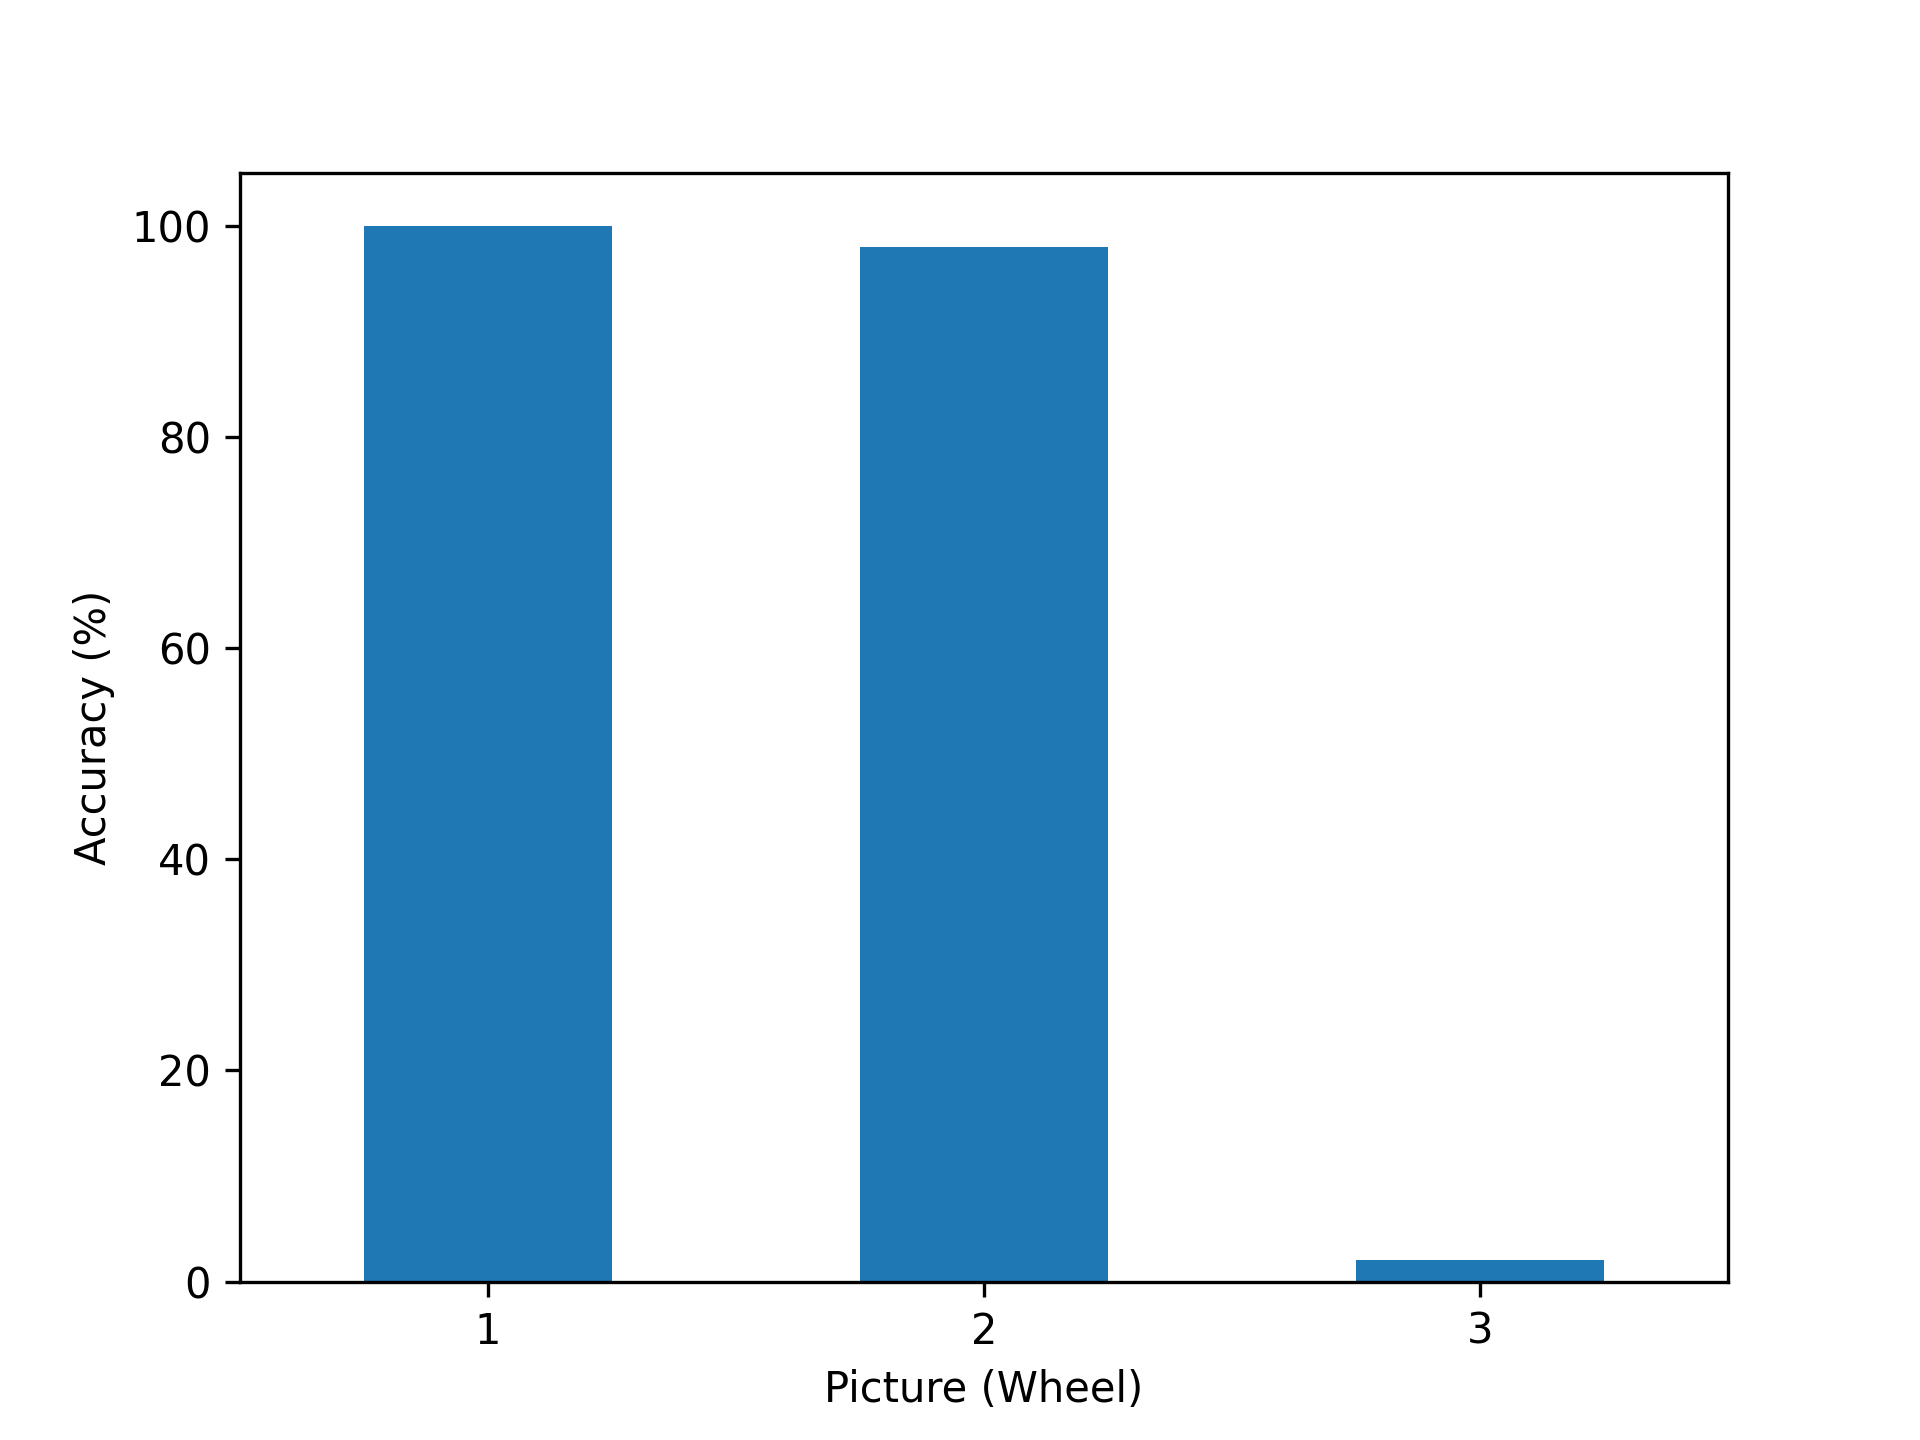
\includegraphics[width=0.5\textwidth]{../Data/wheel-outliers.png}
   \caption{Accuracy Discrepancy Among Images in Whell Class at 14,000 Training Iterations}
   \label{fig:13000-wheel}
\end{figure}

A similar analysis can be drawn for the wheel class, in Figure \ref{fig:13000-wheel} the accuracy score for the three instances of the wheel class at 14,000 training iterations can be observed. Whilst images 1 and 2 received 100 percent and 98 percent accuracy, image 3 displays as a clear anomaly with only 2 percent accuracy. 


\begin{figure}[h]
   \centering
   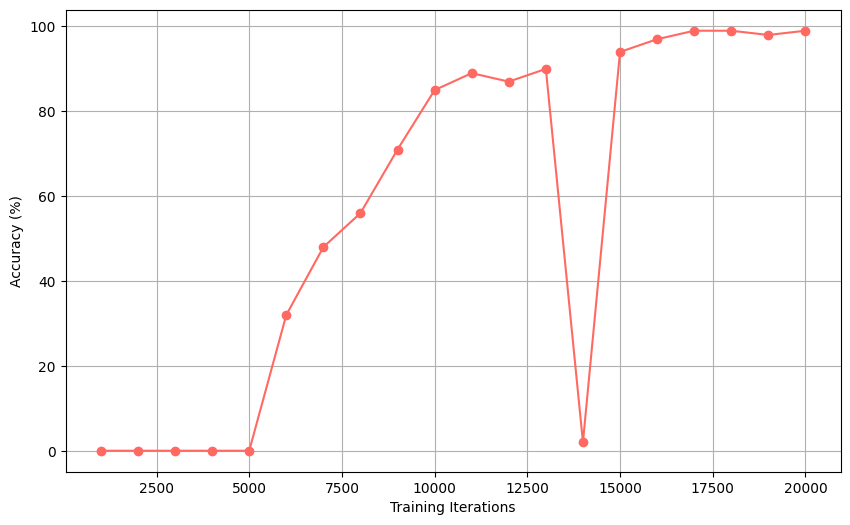
\includegraphics[width=0.5\textwidth]{../Data/wheel_image1_accuracy_vs_iteration.png}
   \caption{Dog Class Image 3 Training Iterations vs. Accuracy }
   \label{fig:image-3-accuracy}
\end{figure}

To further analyse the cause of the anomaly found at 14,000 iterations in image 3, figure \ref{fig:image-3-accuracy} can be utilised, displaying the accuracy of image 3 in the wheel class over 20,000 iterations. This graph illustrates that the given anomaly does not follow the data trend, but rather deviates from the accuracy trajectory, due to its considerably lower accuracy score. Consequently, this data point can also be classified as an outlier, this will be further examined in the discussion chapter. \\
\newpage


\subsection{Distribution of model accuracy across training iterations}

\begin{figure}[h]
   \centering
   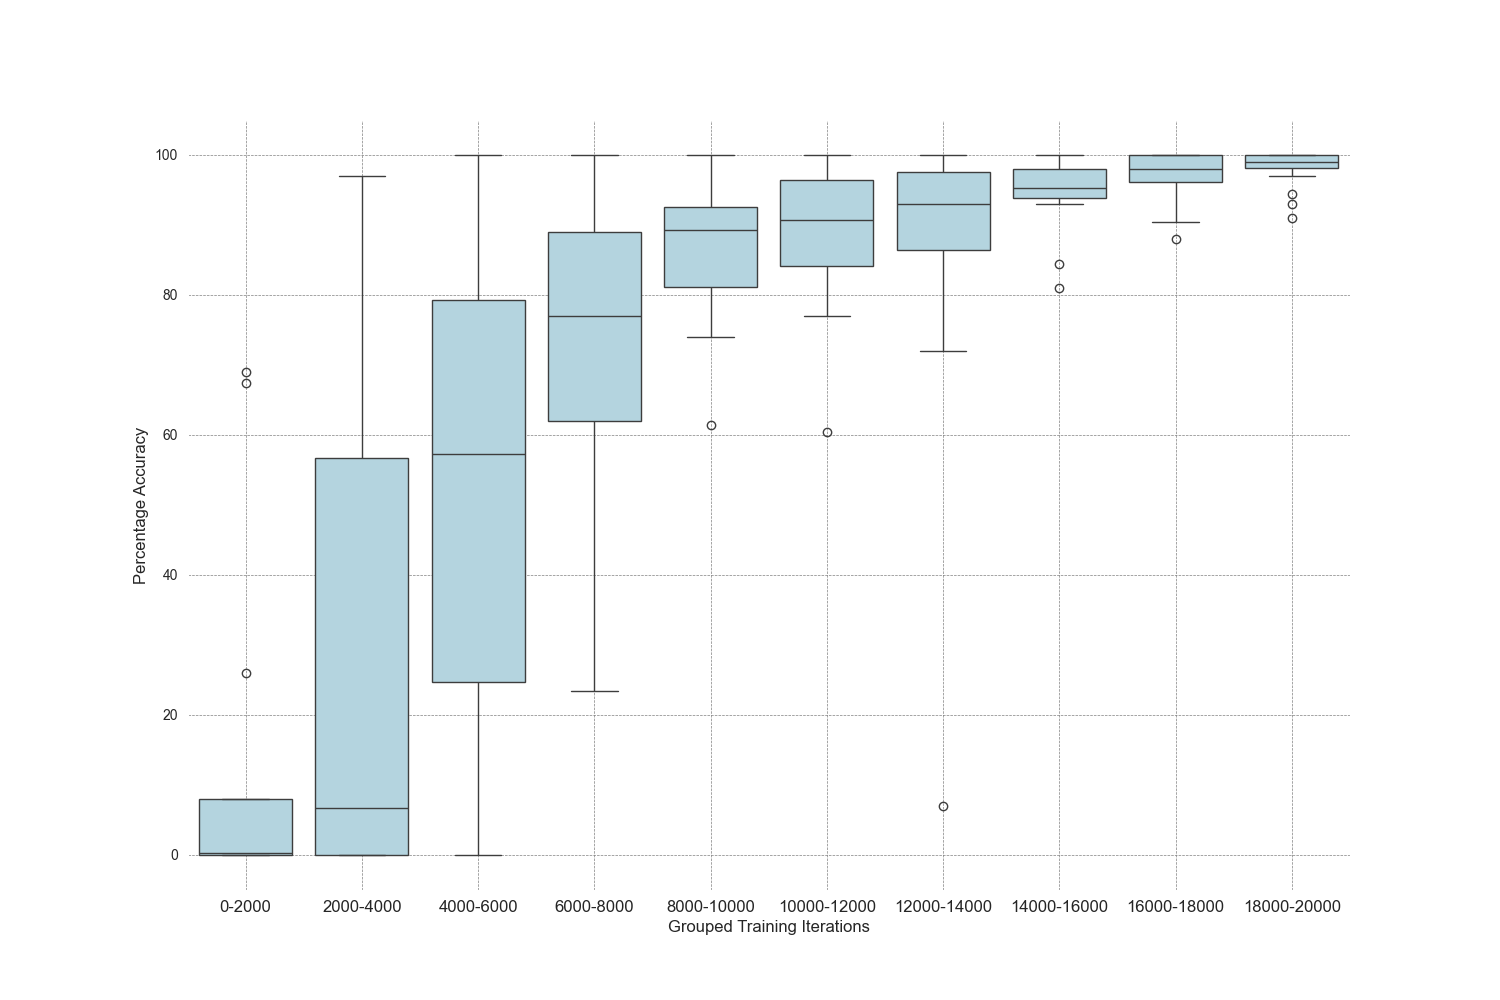
\includegraphics[width=0.9\textwidth]{../Data/box_plot_iteration_vs_accuracy.png}
   \caption{Box Plot of Model Accuracy Across Different Training Iteration Groups}
   \label{fig:Box-plot}
\end{figure}


The following Figure \ref{fig:Box-plot} illustrates a comprehensive overview of the changes in the model's accuracy throughout 20,000 training iterations. It displays the distribution and tendencies of the accuracy throughout the training process in relation to the entire model.\\

Initially, the Figure displays an initial surge in model accuracy up to 4000 iterations. From this point onwards, the median accuracy stabilizes and the variance diminishes in the 4000-12000 training iteration range. Beyond 12000 iterations, there is only minimal change in the median accuracy, signalling the onset of a plateau. Thereafter the graph displays that with further training, only a slight decrease in variance and an increase in median is achieved. \\

One key aspect that the box plot highlights is the changes in data variability throughout the model's training process. Initially, a greater degree of variability is displayed, especially in the grouped 2000-4000 training iteration block. Here the interquartile range (IQR) is notably wider, clearly displaying the greater spread of different accuracy scores.  However, as the training iteration count increases, the range of the spread decreases. The IQR becomes progressively narrower in the higher training iteration groups, indicating a decrease in variability. \\










\section{Discussion}
In the following chapter, the results gathered will be interpreted, focusing on addressing the specified research question. This analysis will enable the hypothesis to be tested, determining whether it holds true or not.


\subsection{Data Interpretation}

The experiment aimed to investigate the relationship between the training iteration count of a machine learning model against the accuracy of a computer vision program. The results illustrated a noticeable correlation between accuracy and the training iteration count. With advancements in the model's training, it was able to continuously improve its accuracy. This demonstrates the machine learning self-improvement as it approaches a state of convergence. Furthermore, it illustrates a strong correlation between the given independent and dependent variables.  \\

When analysing the model's evolution, it is observed that during the initial training phase, the model either failed to identify any objects or did so with a limited accuracy score. This can be justified by the model's unfamiliarity with the objects it is intended to identify, as it is not yet familiar with the given patterns through which it should detect the objects. In the next stage, the model demonstrates rapid development as its accuracy scores vastly increase, displaying an improvement in the model's object detection. This shows the model establishing an understanding of the objects and further developing its pattern-recognising capabilities, resulting in improved accuracy scores. As the experiment progresses into the later stages, the model begins to approach a state of convergence. Additionally, the trade-off between training and accuracy becomes less pronounced. Increased training no longer results in further increased accuracy, demonstrating the reduced effectiveness of the trade-off. Herby also indicates the beginning of a plateauing stage for the accuracy data.   \\ 

Noteworthy is also the weak inverse correlation between the loss and accuracy of the model throughout the training process. This indicates that as the accuracy increases, the loss decreases. The loss is a measure of the errors made by a model \parencite{Baeldung2022}. This also explains the observed inverse correlation. With fewer errors, the lower the loss will be and in return will lead to higher precision, resulting in a higher accuracy score.  \\

% ----- DIP EXPLAINED -----

Additionally, the findings reveal a slight drop in the performance of the model in the later stages of the experiment, 
characterised by a dip in the results. \\

One explanation for this can be overfitting, in which the model excessively adapts to the given training data, compromising the ability to 
adapt to new data such as the test images used. Therefore, after overfitting, the model could obtain lower accuracy scores in comparison 
to scores obtained in previous training iterations. Three causes for overfitting could be noise in the dataset, 
hypothesis complexity, or multiple comparison procedures. Another reason, according to Xue, is "early stopping",
which means that the accuracy of the object recognition model may deteriorate due to noise learning,
which is a pretty strong concept from the 1970s \parencite[1--2]{Xue2019}. \\

Further explanations also could be the model's learning rate or problems with the training data set. If the learning rate is too high, the
model might be taking too large steps in the parameter space and overshooting the optimal solution \parencite{GreatLearningTeam2020}.
Problems with the dataset could be imbalanced in which case the model might become biased towards the majority class \parencite{Brownlee2019a}. 
This imbalance can be seen in Figure \ref{fig:class-usage-in-dataset}. But this imbalance is likely not the cause of the issue since 
"Wheel" has the second highest representation in the dataset, while "Dog" has a relatively low representation, but both classes show the same 
fluctuation in accuracy at roughly the same time. \\

The last option is that the fluctuations could be a result of random chance. Due to the stochastic nature of most optimization algorithms
used in machine learning, the performance of the model can sometimes worsen purely due to random chance \parencite{Brownlee2021}. \\


Notable is also the spread of the data and its variance found in the results as the accuracy improves over time. This is a key aspect of such models for real-world applications, where consistent performance is essential. For instance, in self-driving cars, such deployed models must be able to consistently identify objects with high precision, not just occasionally. Even though the model at times reached high accuracy scores, it was inconsistent and instances of low accuracy scores were recurring, resulting in greater variance. However, in the later training stages,  as the median accuracy increased, the variance reduced, resulting in the lower accuracy scores of the given later stage, still being relatively high and precise predictions by the model.    \\

As revealed in the results section two distinct outliers were discovered in the ‘dog’ and ‘wheel’ image categories. These data points, significantly deviate from the rest. To mitigate the impact such outliers have, a larger pool of data points would be helpful.  \\


\subsection{Hypothesis and Research Question Evaluation}
Following the interpretation of the results obtained, it is of importance, to evaluate the key postulations formed in the hypothesis. It was hypothesised that the accuracy of the model would increase as the training iteration count advanced, this correlation between the two variables of the experiment was portrayed. Further, it was proposed, that during the initial training iterations of the experiment, the data would portray little or no accuracy as the model would be unfamiliar with the patterns it is analysing. This likewise was confirmed by the data. Furthermore, it was predicted that between around 3000 and 12000 iterations the largest growth of accuracy would be discovered, which again was confirmed in the results. \\

A further hypothesis stated that after 80\% accuracy, the data would start plateauing out. This postulation was disproved as the accuracy carried on improving and only in the later stages of the experiment, whilst over 95\% started plateauing out.  Additionally, the hypothesised inverse correlation between loss and accuracy was also confirmed. As the model's accuracy improved, the number of errors decreased, which led to a reduced loss.\\ 

In conclusion, it can be stated that the hypothesis set forth for the experiment was to a high degree accurate and received validation from the data obtained, offering insightful conclusions for the given research question.
\\	

\subsection{Limitations}
The first limitation faced was regarding the constrained data set available. This was portrayed by the model only being evaluated up to 20,000 training iterations, leaving the model's performance thereafter unknown. This meant that there was no data on how the model functions after the 20,000 iterations. This limitation restricted the possibility of evaluating patterns that could be found thereafter.
A further limitation of the given experiment is the limited computing power a M1 Macbook Air offers. Whilst this laptop offers acceptable computing capabilities, it is restricted when it comes to extensive data sets and complex computations. This can have direct effects on the efficiency and depth of the experiment.
The final limitation faced in this experiment concerns itself with the machine learning model created using Apple's Create ML. 
Given the lack of control and insight into the internal functions of Create ML, the possibility of customising the model according to the
requirements is limited. In addition, the use of this closed-source framework has limited the ability to accurately identify the dips 
seen in figure \ref{fig:accuracy-vs-training-iterations} and to accurately investigate the problem. 
Therefore having the given dependency on a pre-designed tool restricts the possible flexibility and addptability of the experiment following the given methodology.  \\

\subsection{Further research}
Following the experiment concerning the relationship between accuracy and training iteration count, further research possibilities emerged. Here two such opportunities will be outlined with a short rationale.  \\

The first further research opportunity concerns itself with the kernel stride length in the computer vision programs' pattern recognition. An investigation could be conducted, experimenting with how different stride lengths impact the accuracy of such a model.   \\

The second area for further research concentrates on speed vs accuracy and the exact, trade-off between these two. This experiment could aim to find an optimal zone in which the training duration is manageable, whilst still aching acceptable accuracy.   \\





\section{Appendix: Raw Output Data from the Experiment}

\begin{table}[h!]
\centering
\begin{tabular}{|c|c|c|c|}
\hline
\textbf{Iteration} & \textbf{Picture 1} & \textbf{Picture 2} & \textbf{Picture 3} \\
\hline
1000 & 0 & 0 & 0 \\
2000 & 0 & 0 & 0 \\
3000 & 0 & 0 & 0 \\
4000 & 20 & 0 & 0 \\
5000 & 34 & 0 & 0 \\
6000 & 52 & 24 & 53 \\
7000 & 63 & 39 & 61 \\
8000 & 74 & 57 & 78 \\
9000 & 88 & 83 & 88 \\
10000 & 93 & 89 & 91 \\
11000 & 94 & 50 & 92 \\
12000 & 95 & 71 & 91 \\
13000 & 96 & 69 & 95 \\
14000 & 95 & 75 & 93 \\
15000 & 95 & 83 & 94 \\
16000 & 97 & 85 & 95 \\
17000 & 98 & 90 & 96 \\
18000 & 97 & 97 & 98 \\
19000 & 99 & 96 & 99 \\
20000 & 98 & 99 & 100 \\
\hline
\end{tabular}
\caption{Iteration and Accuracy for Boat}
\end{table}

\begin{table}[h!]
\centering
\begin{tabular}{|c|c|c|c|}
\hline
\textbf{Iteration} & \textbf{Picture 1} & \textbf{Picture 2} & \textbf{Picture 3} \\
\hline
1000 & 1 & 26 & 1 \\
2000 & 1 & 26 & 1 \\
3000 & 2 & 48 & 2 \\
4000 & 3 & 57 & 3 \\
5000 & 47 & 67 & 1 \\
6000 & 67 & 69 & 45 \\
7000 & 78 & 78 & 47 \\
8000 & 75 & 75 & 67 \\
9000 & 75 & 87 & 75 \\
10000 & 88 & 93 & 88 \\
11000 & 87 & 78 & 92 \\
12000 & 88 & 83 & 87 \\
13000 & 12 & 87 & 89 \\
14000 & 89 & 93 & 89 \\
15000 & 92 & 93 & 92 \\
16000 & 95 & 94 & 95 \\
17000 & 96 & 89 & 97 \\
18000 & 98 & 92 & 98 \\
19000 & 98 & 93 & 99 \\
20000 & 99 & 93 & 99 \\
\hline
\end{tabular}
\caption{Iteration and Accuracy for Dog}
\end{table}


\begin{table}[h!]
\centering
\begin{tabular}{|c|c|c|c|}
\hline
\textbf{Iteration} & \textbf{Picture 1} & \textbf{Picture 2} & \textbf{Picture 3} \\
\hline
1000 & 49 & 2 & 51 \\
2000 & 86 & 2 & 87 \\
3000 & 93 & 65 & 95 \\
4000 & 95 & 74 & 99 \\
5000 & 96 & 96 & 100 \\
6000 & 98 & 94 & 100 \\
7000 & 98 & 94 & 100 \\
8000 & 96 & 97 & 100 \\
9000 & 100 & 91 & 100 \\
10000 & 100 & 98 & 100 \\
11000 & 100 & 98 & 100 \\
12000 & 100 & 98 & 100 \\
13000 & 100 & 100 & 100 \\
14000 & 99 & 93 & 100 \\
15000 & 100 & 98 & 100 \\
16000 & 100 & 97 & 100 \\
17000 & 100 & 100 & 100 \\
18000 & 100 & 100 & 100 \\
19000 & 100 & 99 & 100 \\
20000 & 100 & 99 & 100 \\
\hline
\end{tabular}
\caption{Iteration and Accuracy for Person}
\end{table}

\begin{table}[h!]
\centering
\begin{tabular}{|c|c|c|c|}
\hline
\textbf{Iteration} & \textbf{Picture 1} & \textbf{Picture 2} & \textbf{Picture 3} \\
\hline
1000 & 0 & 0 & 0 \\
2000 & 0 & 0 & 0 \\
3000 & 0 & 0 & 0 \\
4000 & 0 & 0 & 5 \\
5000 & 0 & 0 & 51 \\
6000 & 51 & 0 & 64 \\
7000 & 62 & 0 & 79 \\
8000 & 64 & 47 & 77 \\
9000 & 73 & 52 & 82 \\
10000 & 71 & 77 & 85 \\
11000 & 83 & 78 & 79 \\
12000 & 84 & 76 & 88 \\
13000 & 82 & 73 & 92 \\
14000 & 81 & 82 & 91 \\
15000 & 93 & 84 & 93 \\
16000 & 96 & 79 & 95 \\
17000 & 99 & 87 & 93 \\
18000 & 100 & 89 & 93 \\
19000 & 100 & 91 & 94 \\
20000 & 99 & 91 & 95 \\
\hline
\end{tabular}
\caption{Iteration and Accuracy for Plant}
\end{table}


\begin{table}[h!]
\centering
\begin{tabular}{|c|c|c|c|}
\hline
\textbf{Iteration} & \textbf{Picture 1} & \textbf{Picture 2} & \textbf{Picture 3} \\
\hline
1000 & 0 & 0 & 0 \\
2000 & 0 & 0 & 0 \\
3000 & 0 & 22 & 0 \\
4000 & 48 & 36 & 0 \\
5000 & 66 & 58 & 0 \\
6000 & 81 & 77 & 32 \\
7000 & 89 & 81 & 48 \\
8000 & 85 & 83 & 56 \\
9000 & 91 & 90 & 71 \\
10000 & 93 & 91 & 85 \\
11000 & 95 & 96 & 89 \\
12000 & 96 & 96 & 87 \\
13000 & 95 & 94 & 90 \\
14000 & 100 & 98 & 2 \\
15000 & 99 & 98 & 94 \\
16000 & 100 & 97 & 97 \\
17000 & 100 & 98 & 99 \\
18000 & 98 & 99 & 99 \\
19000 & 100 & 100 & 98 \\
20000 & 100 & 99 & 99 \\
\hline
\end{tabular}
\caption{Iteration and Accuracy for Wheel}
\end{table}


\begin{table}[h!]
\centering
\begin{tabular}{|c|c|}
\hline
\textbf{Iteration} & \textbf{Loss} \\
\hline
1000 & 10.92 \\
2000 & 10.91 \\
3000 & 9.96 \\
4000 & 9.21 \\
5000 & 8.69 \\
6000 & 8.26 \\
7000 & 7.86 \\
8000 & 6.91 \\
9000 & 7.8 \\
10000 & 7.35 \\
11000 & 7.1 \\
12000 & 6.87 \\
13000 & 6.61 \\
14000 & 6.44 \\
15000 & 6.33 \\
16000 & 6.09 \\
17000 & 5.92 \\
18000 & 5.75 \\
19000 & 4.77 \\
20000 & 5.74 \\
\hline
\end{tabular}
\caption{Loss per Iteration}
\end{table}









\end{document}
	
\printbibliography[title=References]


	
	
	
	
	
	
	
	
	
	
	
	
	
	
	
	
	
	
	
	
	
	
\end{document}          
